\documentclass{standalone}
\usepackage{mathpazo}
\usepackage{siunitx}
\usepackage{tikz}
\usetikzlibrary{shapes}
\begin{document}


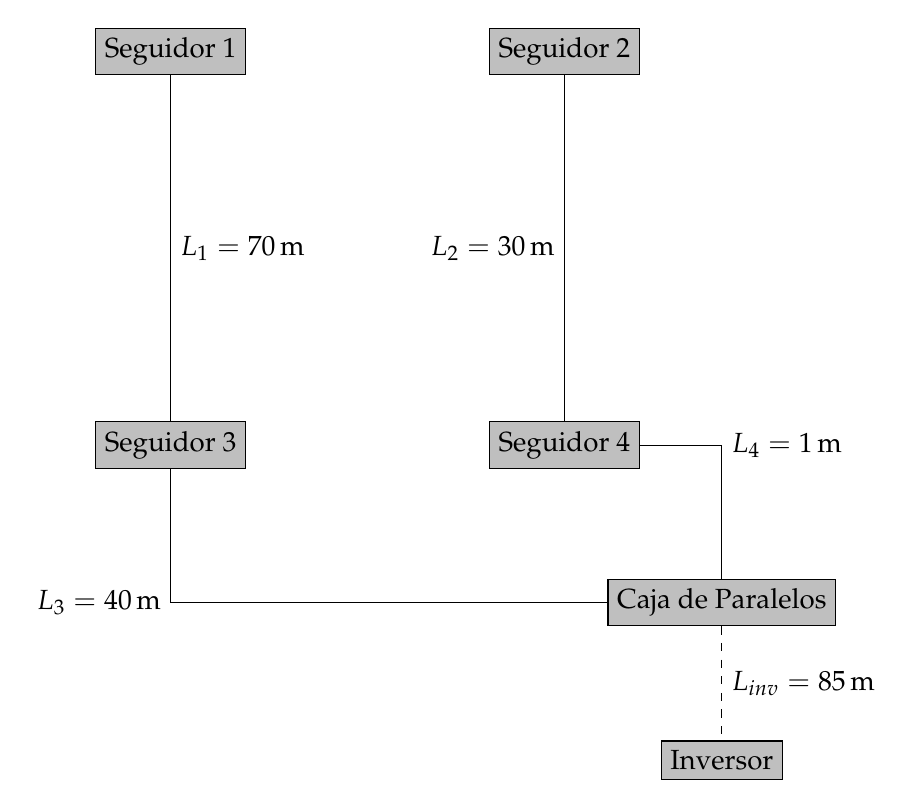
\begin{tikzpicture}
  \node[draw, fill = lightgray] (S1) at (0, 5) {Seguidor 1};
  \node[draw, fill = lightgray] (S2) at (5, 5) {Seguidor 2};
  \node[draw, fill = lightgray] (S3) at (0, 0) {Seguidor 3};
  \node[draw, fill = lightgray] (S4) at (5, 0) {Seguidor 4};
  \node[draw, fill = lightgray] (CP) at (7, -2) {Caja de Paralelos};
  \node[draw, fill = lightgray] (Inv) at (7, -4) {Inversor};

  \draw
  (S1) -- (S3) node[midway, right] {$L_1 = \qty{70}{\meter}$}
  (S2) -- (S4) node[midway, left] {$L_2 = \qty{30}{\meter}$}
  (S3) |- (CP) node[midway, left] {$L_3 = \qty{40}{\meter}$}
  (S4) -| (CP) node[midway, right] {$L_4 = \qty{1}{\meter}$};
  \draw [dashed]
  (CP) -- (Inv) node[midway, right] {$L_{inv} = \qty{85}{\meter}$};

\end{tikzpicture}

\end{document}